
%% bare_conf.tex
%% V1.3
%% 2007/01/11
%% by Michael Shell
%% See:
%% http://www.michaelshell.org/
%% for current contact information.
%%
%% This is a skeleton file demonstrating the use of IEEEtran.cls
%% (requires IEEEtran.cls version 1.7 or later) with an IEEE conference paper.
%%
%% Support sites:
%% http://www.michaelshell.org/tex/ieeetran/
%% http://www.ctan.org/tex-archive/macros/latex/contrib/IEEEtran/
%% and
%% http://www.ieee.org/

%%*************************************************************************
%% Legal Notice:
%% This code is offered as-is without any warranty either expressed or
%% implied; without even the implied warranty of MERCHANTABILITY or
%% FITNESS FOR A PARTICULAR PURPOSE! 
%% User assumes all risk.
%% In no event shall IEEE or any contributor to this code be liable for
%% any damages or losses, including, but not limited to, incidental,
%% consequential, or any other damages, resulting from the use or misuse
%% of any information contained here.
%%
%% All comments are the opinions of their respective authors and are not
%% necessarily endorsed by the IEEE.

\documentclass[a4paper]{article}


\usepackage{natbib}
\usepackage{amsmath}
\usepackage{subfigure}
\usepackage{graphicx}
\usepackage{graphics}
\usepackage{pstricks,pstricks-add}
\newcommand{\figurepath}{Figures}

\newcommand{\titlesize}{\fontsize{16pt} \selectfont}


\begin{document}
%
% paper title
% can use linebreaks \\ within to get better formatting as desired
\title{\titlesize \bf Adaptive Character Motion Synthesis By Qualitative Approach}

\author{
Fangde Liu\\
\\National Center For Computer Animation\\Media School\\
\\Bournemouth University\\
Email: fliu@bmth.ac.uk
\and
Xiaosong Yang\\
NCCA\\Media School\\
Bournemouth University\\
xyang@bournemouth.ac.uk
\and
Jianjun Zhang 
NCCA\\Media School\\
Bournemouth University\\
jzhang@bournemouth.ac.uk
}


% author names and affiliations
% use a multiple column layout for up to three different
% affiliations
%\author{\IEEEauthorblockN{Fangde Liu}
%\IEEEauthorblockA{National Center For Computer Animation\\Media School\\
%Bournemouth University\\
%Email: fliu@bmth.ac.uk}


%\and

%\IEEEauthorblockN{Xiaosong Yang}
%\IEEEauthorblockA{NCCA\\Media School\\
%Bournemouth University\\
%xyang@bournemouth.ac.uk
%}
%\and
%\IEEEauthorblockN{Jianjun Zhang}
%\IEEEauthorblockA{NCCA\\Media School\\
%Bournemouth University\\
%jzhang@bournemouth.ac.uk
%}
%}

% conference papers do not typically use \thanks and this command
% is locked out in conference mode. If really needed, such as for
% the acknowledgment of grants, issue a \IEEEoverridecommandlockouts
% after \documentclass

% for over three affiliations, or if they all won't fit within the width
% of the page, use this alternative format:
% 
%\author{\IEEEauthorblockN{Michael Shell\IEEEauthorrefmark{1},
%Homer Simpson\IEEEauthorrefmark{2},
%James Kirk\IEEEauthorrefmark{3}, 
%Montgomery Scott\IEEEauthorrefmark{3} and
%Eldon Tyrell\IEEEauthorrefmark{4}}
%\IEEEauthorblockA{\IEEEauthorrefmark{1}School of Electrical and Computer Engineering\\
%Georgia Institute of Technology,
%Atlanta, Georgia 30332--0250\\ Email: see http://www.michaelshell.org/contact.html}
%\IEEEauthorblockA{\IEEEauthorrefmark{2}Twentieth Century Fox, Springfield, USA\\
%Email: homer@thesimpsons.com}
%\IEEEauthorblockA{\IEEEauthorrefmark{3}Starfleet Academy, San Francisco, California 96678-2391\\
%Telephone: (800) 555--1212, Fax: (888) 555--1212}
%\IEEEauthorblockA{\IEEEauthorrefmark{4}Tyrell Inc., 123 Replicant Street, Los Angeles, California 90210--4321}}




% use for special paper notices
%\IEEEspecialpapernotice{(Invited Paper)}




% make the title area
\maketitle


\begin{abstract}
%\boldmath
Adaptive motion synthesis normally involves very complicate computation from physical simulation.  However based on the biological research, the neural system of human being and animals only take very little effect to control their motion. Instead of controlling each part of its body, natural life only maintains or tweaks some qualitative properties of its motion system to finish very complicate interaction with environment. Inspired by this special working pattern, in this paper, we proposed a new efficient adaptive motion synthesis method based on the qualitative control theory. It involves only very little computation to control the qualitative properties of motion. Adaptive motion control is achieved through manipulating the topological structure of the dynamic system to enhance the structural stability, rather than counteracting the perturbation effects. Compared with current simulation method, our algorithm is more computational efficient and has the potential to be accelerated by GPU.
\end{abstract}

{\bf keywords:}

Charater Motion Synthesis, Qualitative Dynamic, Physics Based Animation





\section{Introduction}

Human being has very high level of perception sensitivity on motions. From the variety in motion details, humans can infer the changes in mental states, health conditions or even the surrounding environment. This makes Character Motion Synthesis (CMS) a very difficult task to deal with. Sometimes a very tiny change in the character motion will lead to very bad motion. In the past two decades, lots of work has been published to achieve the target of generating realistic character motions. In industry, high quality motions are still majorly generated by animator's manual work. Because of the complicate structure of each character, a large number of joints need animator to tweak and setting key frames. To make things worse, it is very difficult to reuse these motion data. When the environment or the character changed, the animators have to manually design new motions.

To save animator from these tedious manual works, many researchers are trying to generate lifelike motions automatically by simulating the dynamics of body, environment and the neural control system. However since each virtual character is full of redundant degree of freedom, it not only increases the computational load, but also makes the solution nondeterministic. 

In Biology, lots of researchers have been working on the secret of motions for centuries. They found out some important features for the motions of live creatures:

\textbf{Adaptive} 
Natural motions are adaptive to the changes in the environment or body conditions. For example, a human being can easily adjust its walking motion according to different terrains.

\textbf{Agile}
The reaction of human and most animals are very fast. Even in a very complicated changing environment, human can change their motions in real time. However from the biology research, the simple functionality and slow processing speed of human neural system make it almost impossible to solve complex motion control problem in a real time. 

\textbf{Energy Efficient}
According to Darwin's Theory of Evolution, a natural motion should be energy efficient. Live creatures spent far less energy than we expected. An example is that the energy consumed by human walking is only 10\% of that for a robot of the same scale.

Since all the simulation methods are trying to accurately simulate the physical property of character motion, it is very hard for them to solve the complicated adaptive motion through simple computation. The above three important features are very difficult to achieve by current CMS methods.
In this paper, we will bring in the Qualitative Control Theory (QCT) to tackle motion synthesis problem. Based on QCT, a natural motion is in nature a structural stable autonomous system, and the key factor of motor control is the topological structure of the dynamic motion systems. So in our method, only the qualitative properties of motions are controlled. Adaptation to different environment or changing of character conditions will be produced automatically with very little control effort. All the above three natural motion features can be achieved from our system. Our method works especial efficient for repetitive and low energy motion tasks which are most challenging for motion synthesize. Compared with other methods, our approach is more computational efficient and has the potential to be further accelerated by GPU.

\section{Related Work}

\subsection{Dynamic Motion Synthesis and Control}
Dynamic Motion Synthesis  tries to synthesize character motion through physical simulation of the mechanic structure of character body which is usually modelled as a linked rigid body system \citep{Baraff1994,Mirtich1996,Stewart2000}. Since many real physical properties are considered in the computation, the generated motion are normally physical feasible. However the most difficult task for those methods is to design a efficient control system to simulate the functionality of a real biological neural system. Some early research applied classical control methods like PD controller \citep{Raibert1991} for locomotion. Later research \citep{Hodgins1995} applied the same method for different tasks like running, bicycling, vaulting and balancing. Limit Circle Control(LCC) \citep{Laszlo1996} provides an alternative method for lower energy locomotion animation. However both the classical PD controller and Limit Circle Controller predefined motion trajectories and eliminated perturbations. This make them not good at generating motion adaptation.

Because lots of degrees of freedom are involved in the whole body simulation, in most cases, motion solutions are not unique. Many optimization methods have been applied to choose the ``best'' motion. For dynamic methods, a reasonable choice is to minimize the energy cost~$V$, such that 
\[
\textbf{V}=\int_{t0}^{t1}F_{a}(x)^2dt
\]
where $F_{a}$ is the active force generated by actuators like motors or muscles. This is introduced to CMS research as the influential Spacetime Constraints\citep{Witkin1988}, and serve as the foundation for many modern CMS research. \citet{Jain2009} provides an example for locomotion;  \citet{BalanceControl} find a method for balance maintaining movement. \citet{Liu2009} proposed a method for object manipulating animation.

The Spacetime method may modify the motion trajectory and in nature it solve the problem through variational optimization. However it faces several key problem.\\
\textbf{Efficiency}
In many cases, it will take very long time to find the "best" solution and there is no guarantee the optimal solution can be achieved. And for complex body structures the computation will takes prohibitive long time \citep{Anderson2001}. Optimization techniques like time window and multi-grid techniques are proposed by \citet{Cohen1992} and \citet{Liu1994}. Very a few research \citep{Popovi'c1999} proposed Spacetime Constraint for full body dynamic animation.\\
\textbf{Sensitive and Overspecific}
Current numeric methods are very sensitive to model accuracy and initial conditions. Precise model for both the environment and body have to be prebuilt. \citet{Liu2005} points out that spacetime constraint methods only suit high energy motions like jumping and running; for low energy motion tasks like walking the result doesn't looks nature. This is mainly because the muscle effects are neglected. Motions like heart beating, breathing, or motions of other animals such as the swimming of fish and jellyfish, flying of birds have not been synthesized with dynamic methods for the lack of a feasible dynamic model. 


\subsection{Biological Research}
In biological research, motor control is an age old problem full of paradoxes. Motor control in nature is a complex process involving many chemical, electrical and mechanical effects. So most of Dynamic motion synthesis methods tries to simulate the reality through very complicated computation. However this is very opposite to the characteristics of the neural systems of real creatures \citep{Glynn2003}: \\
\textbf{Time Delay}
Neural signal transmitting speed is very slow; and there is a long delay between neural signal firing and force generation in muscles.\\ 
\textbf{Noisy}
Besides the delay and low speed transition, the neural signals are also noisy. The body structure and environment are also nonlinear, noisy and time varying. \\
\textbf{Limited Activity}
Current research evidences and common life experience show that motor control involves little control effort. Many experiments show motion can happen even without brain input. 

Despite the complexity of body structures and environment, the natural motor control strategy seems relatively simple involving vey little computational work. In many animals, the active neural structure in motor control is the Central Pattern Generator(CPG) which generates rhythmic signals. There are many experimental researches in robotics and biomechanics succeeded in controlling some motion with very simple strategy\citep{nishikawa2007neuromechanics}. \textbf{Uncontrolled Manifold Hypothesis} method even proposed that some DOFs are not controlled and freely influenced by the environment \citep{latash2008neurophysiological}. The\textbf{Equilibrium Point Hypothesis} method suggests that what the neural systems controls is not trajectory, but the final position. The \textbf{Impedance Control Hypothesis}\citep{hogan1985ica} method refines the idea of EPH by providing an explanation for effects of the extra DOFs. Impedance Control proposed the extra DOFs provide a way to control the stability and admittance of final postion according to the motion purpose. \textbf{Morphological Computation Theory} \citep{nishikawa2007neuromechanics,Pfeifer2005} thinks both the body structure and the environment play a crucial role in  motor control, basic motion patterns are generated by body and environment, the neural systems only  maintains or tweaks such motion patterns.

The biological ideas provide space for an efficient motion adaptation, but the theory are incomplete and mainly for explaining experiment results. There is a big knowledge gap to turn it into a sound control theory.

\section{Qualitative Dyanmic For CMS}
\subsection{Qualtiative Mechanical Theory}
The Qualitative Control Theory is a mathematical description of the MCT
In qualitative control theory the  basic patterns of motion are called \textbf{motion primitive}.
In mathematic terms, motion primitives are \textbf{structural stable autonomous systems}

\subsubsection{Basic Concepts of Qualitative Dynamics} 
Qualitative Dynamics can be traced back to Poincare\citep{Poincar'e1899,Poincar'e1885} and recently developed by the Smale School.
Please refer to other books and lectures  such as \citep{abraham1978foundations}for introduction in details.

The configuration of system is described using state value in the state space.
we represent the state of a system as a vector $q$,  $M$ is the state space, which is a manifold.
The motion trajectory over time is $q(t)$.
For a dynamic system, $q(t)$ is usually in the form of  ordinary differential equation. 
\begin{equation}
\dot{q}=F_{u}(q)=F(q,u),q\in M
\label{eq:ode}
\end{equation}
where $u$ is the control effort. 
$F$ is determined by the system's natural property.
If $u=0$,  no control effort is applied.
Such systems are \textbf{autonomous systems}.
For every point $q \in M$, 
$F$ and $u$ determines a derivative vector $\dot{q}$. 
All the vectors over the full space of $M$ form the \textbf{vector field} $V$. 
There is a corresponding geometry structure for Equation \eqref{eq:ode}, a differentiable manifold.
The motion trajectory can be found by apply the integral operation on the vector field.
The result trajectory is defined as \textbf{flow} $\Phi$, all the flows form another geometry structure,
the \textbf{phase portrait}, which illustrates all the possible motions of the dynamic system.


On the phase plane,
Flows can only intersect at some special position.


\textbf{Fix Point} The first type of intersection is fix point or equilibrium point~$q_{e}$.
\[
	H(q_{e})=0
\]

\textbf {Period Flow} Another type of intersection is a periodic flow. For any point $q$ on the circle, we have
\[
	H(q(0))=H(q(T))
\]


Intersections like fixed point and are also called \textbf{equlibria}, 

At each \textbf{equilbria}, 
the local space can be divided into three subspace of submanifold: centre submanifold, stable manifold, and unstable submanifold.

\textbf{centre submanifold}
If a flow $\theta$ pass through a point $m$ on centre submanifold $W_{c}$,
flow$\theta$ will remain on the Centre Manifold 
\[
\theta_{c}(t) \in W_{c}, t \in R
\]
 An equilibria must be on center manifold.

 
\textbf{stable submanifold}
For the flow $\theta_{s}$ passes through a point $m$ on stable submanifold $W_{s}$, the flow will finally converge to a nonwandering point on centre submanifold.
\[
\theta_{s}(+\infty)=\theta_{c}
\]

\textbf{unstable submanifold}
For the flow passes through a point $m$ on unstable submanifold $W_{u}$, the flow will be repelled from the nonwandering points on centre manifold.
An alternative perspective is the inverse of the flow converge to nonwandering point. 
\[
\theta_{u}(-\infty)=\theta_{c}
\] 



For nonlinear system, globally, the shape of stable and unstable submanifold may be bending and connect with itself or each other.
The equilibra and its connectivity of sub manifolds form a topological structure.
The phase plane is divide into different regions,result in a cellular structure.
In each region,there is only one attractor, all the flow in this region will converge to the attractor.
and the corresponding region is called \textbf{basin of attraction}.
\subsubsection{Motion Adaptation and Stability}
A mechanical system can be extremely stable without any control effort. 
This kind of stability is rough stability or structure stability \citep{Andronov1937}.
Rough stability or structure stability is determined by the topology structure of the system\citep{Jonckheere1997}.

Motions vary greatly, this makes it difficult to define motion and tell it from another.
In Qualitative Control Theory, motion should be defined by the topological structure of the coresponding differetial equation.
From topology viewport, motion adaptation can be modelled as homeomorphism.
Homeorphic flows can be generated if the differentiable manifolds are homeomorphic, which means they share the same topological structure,but different shape.

Structure stable autonomous systems have the ability to maintain its topology structure under perturbations.
They generated homeorphic flows while keep the qualitative property, thus the resulting motion is adaptive but qualitatively maintained.

In fact, the effects of control and perturbation can be modelled in the same way.
An autonomous dynamic system is represented as,  
\[
\dot{q}=H(q)
\]
Considering the control and perturbation, the system will be changed into
\[
\dot{q}=H^{'}(q)=H(q)+f(q,t)
\]
Where $f(q,t)$ is used to model both the control and perturbation.

Geometrically, the effect of $f(q,t)$ can be seen as a deformation to the trajectory $q(t)$ on the phase plane.
\[
q^{'}=\Theta(q)
\]
such that 
\[
H^{'}(q)=H(\Theta(q))=H(q^{'})
\]


In Qualitative Control Theory, only final motion results are concerned, 
In mathematical viewport, only the attractors of flows are controlled, while the flow itself is not concerned in motion control.
Also, according two the type of attractors, motion can be group into two groups.

\textbf{Discrete Motion}
Such motions have fixed attractors, typical motions include posture control and picking up motion of the arm.

\textbf{Peridotic Motion}
Such motion have periodic attractors, typical motion include walking, running and heartbeating.

Motions are made up of motion primitives.
Neural control system tweaks the basic motion primitives to achieve specific objective.


Qualitative Control Theory preserve the natural motion features.

\textbf{Adaptive}
Using this method, 
different perturbations will result in different motions. 
Motion will vary with the environment change.

\textbf{Efficient}
Motion will be generated passively and follow the least energy path.

\textbf{Agile}
QCT does not rely on high precise calculation.
Topological structure can be manipulated and maintained by some very simple methods.


\subsection{CPG and Entraintment}
In nature, an animal's body and environment can be extremely complex. 
It leads to high dimensional manifolds with complicated topological structure. 
For CMS application, one question is the whether complex system can be controlled with a simple method.
Biology Research suggested that the motion is mainly controlled by the Central Pattern Generator, which is a small autonomous network that generating rhythmic signals.
The existence of CPG is very common, primitive animals like lamprey and fish, to high level animals like bird, mammal and human\citep{Cohen1988}.
The idea of control motion by rhythmic signals can be modelled as entrainment \citep{Gonz'alez-Miranda2004}.
In this section, we provide the understanding of biological entrainment in the viewport of  Qualitative Control Theory.


\subsubsection{The Biological Entraintment}
Entrainment is the phenomenon that two coupled oscillator systems oscillate in a synchronize way. 
Although the mechanism can be very complex, the phenomenon is universal. 
The classic example shows individual pulsing heart muscle cells.
When they are brought close together, they begin pulsing in synchrony. 

Entrainment will happen when coupling two oscillators with similar oscillation frequencies but with very different characteristics. 
A simple explanation is that energy fluctuates between the two oscillating system.

Given two systems,
\[
\dot x=f(x)
\]
\[
\dot y=g(y)
\]
when two oscillation systems couple, the behaviour of both systems will change. 
The coupled system can be presented with the following equation
\begin{eqnarray}
\dot x=f(x)+m*g(y) \label{eq:couple1}\\
\dot y=g(y)+n*f(x) \label{eq:coule2}
\label{eq:couple}
\end{eqnarray}

where $m$,and $n$ are coupling coefficients. 
When $m$ is large, the behaviour of equation\eqref{eq:couple1} is more dominated by the second term $m*g(y)$. 
This can be seen as a forced oscillation system. 
Even $m$ is small, behaviour of equation\eqref{eq:couple1} can be changed qualitatively.
For some cases, stability can be enhanced and chaotic behavior can be suppressed.


The entrainment model can be applied to CMS, if we took the neural oscillator as $f(x)$ and body as the mechanical oscillator $g(x)$.
The properties of mechanical oscillator can be controlled by the oscillation property of the neural system; the oscillation of mechanical system can be controlled by the oscillation of neural system.
If we increase $n$, we can expect that mechanical oscillators shows the behaviour of neural oscillators. 
Entrainment can help to boost the stability of the mechanical oscillation.
When the mechanical oscillation is disrupted but the neural oscillation remains, after the perturbation is removed, the undisrupted neural oscillation can drive the disrupted mechanical oscillation back to normal.



\subsubsection{The Structural Stable Oscillation of the Neural System}
One extensively studied oscillation model is developed by \citet{neurooscillation}. 
The mathematical presentation is as follows:
\begin{eqnarray}
\tau_{1} \dot{x_{1}}&=&c-x_{1}-\beta v_{1}-\gamma [x_{2}]^{+}-\sum_{j}h_{j}[g_{j}]^{+}\\
\tau_{2} \dot{v_{1}}&=&[x_{1}]^{+}-v_{1}\\
\tau_{1} \dot{x_{2}}&=&c-x_{2}-\beta v_{2}-\gamma [x_{1}]^{-}-\sum_{j}h_{j}[g_{j}]^{-}\\
\tau_{2} \dot{v_{2}}&=&[x_{2}]^{+}-v_{2}\\
y_{i}&=&\mbox{max}(x_{i},0)\\
y_{out}&=&[x_{1}]^{+}-[x_{2}]^{+}=y_{1}-y{2}
\label{eq:matsuta}
\end{eqnarray}
where $x$ and $v$ are state variables of the oscillator, $\tau$,$c$,$\beta$,$\gamma$ are parameters of the oscillator.

Matuoka oscillator is an autonomous oscillator; it can begin to oscillator without any control effort.
It is also adaptive; entrainment behaviour can happen between one Matuoka oscillator and different oscillators. 
But because of the nonlinear properties, its behavior is not completely understood. 
Matsuta\citep{Matsuoka1987} explains the adaptive properties from the location of the roots of  characteristic equation. 
Wilimas\citep{Williamson1998} explains the properties in frequency domain.
In our research, we find some important properties of neural oscillator by investigating the phase portrait.


Basically, neural oscillator shows three important properties:

\textbf{Simple Structure}
The topology structure of neural oscillator is simple, 
it includes one  attractive limit circle and one fix repellor.

\textbf{Large Basin of Attraction}
All the simulations we carried out converged to the same limited circle.

\textbf{Fast Converging Speed}
In most of the case, the flow will converge to the limit circle within one period time.

Features above are shown in \figurename \label{fig:matsuta oscilation}.
\begin{figure}[!h]
\centerline{\subfigure[time state]{
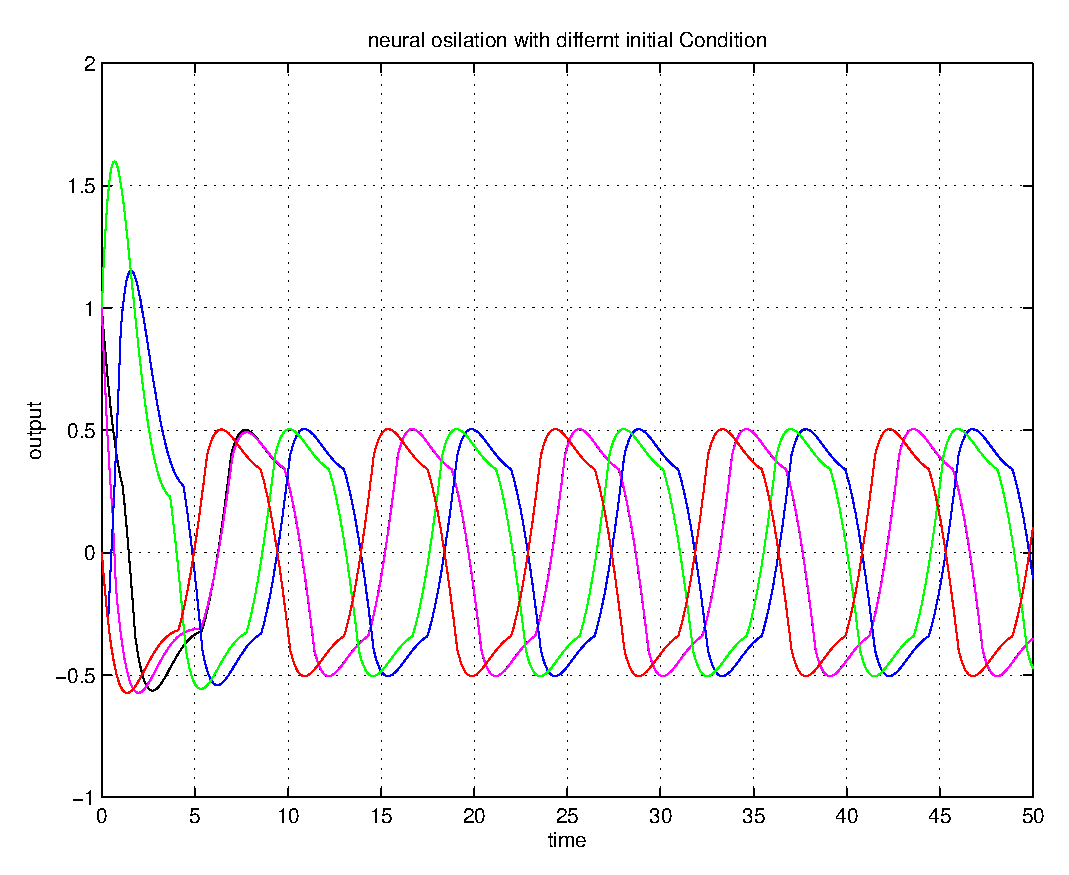
\includegraphics[width=1.5in]{\figurepath/neural_attraction.eps}
\label{fig:time_timeAttraction}
}
\hfill
\subfigure[Phase Portrait]{
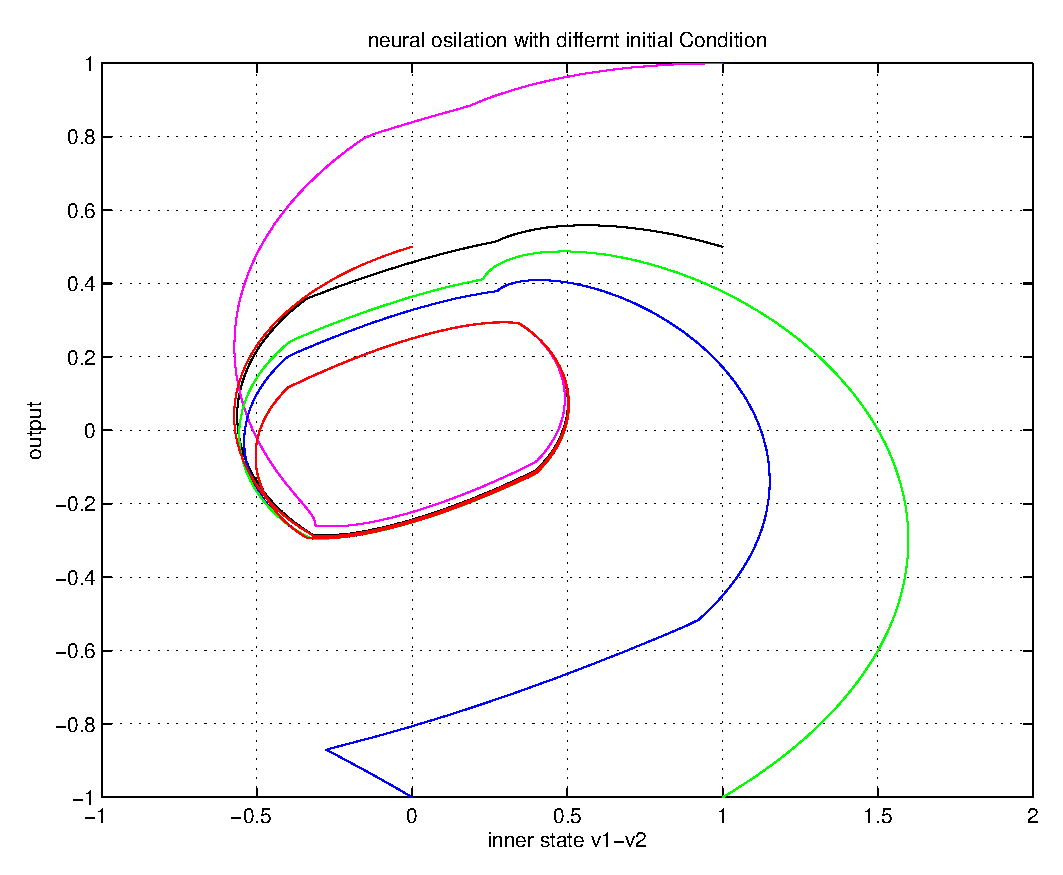
\includegraphics[width=1.5in]{\figurepath/neural_attraction_phase.eps}
\label{fig:phase_attraction}
}
}
\caption{Matsuta Oscilator}
\label{fig:matsuta oscilation}
\end{figure} 
The large area of basin of attraction means the final behavior is totally determined by parameters. 
Initial conditions will have no effects on the final oscillation. 
The converging speed can be seen as quick recovery ability.
When an impulse perturbation happens, it will recover in one period time.
These properties are very valuable in CMS research. 
Matuskota Oscillator is a structure stable autonomous oscillator.
An intuitive idea is that we couple the neural oscillator with mechanical oscillator of body and environment, thus tune the motion a structual stable one

\section{Application to Bipedal Walking}
Bipedal walking is a common motion task and has been well studied by many research communities, including robotic \cite{Raibert1986}, artificial intelligence and biology as well as computer graphic research.
From experience, walking involves little reasoning activity, this idea is supported by the biology research that the number of neurons that take part in the lower limb control is very limited, much less than arm, hand and even tongue.
While for artificial system, robust bipedal walking is difficult to achieve. 
Many control method has been tried, but none of them shows comparable performance with human walking. 
In dynamic research,natural looking gaits can be generated by passive method.
There have been a series of passive dynamic walking machine\citep{McGeer1990,McGeer1990a}. 
If we put a passive walking machine on a slope, without any effort, it can walk down the slop. 
However the stabilities are very fragile. 
Passive walking can only be maintained when walking down a specific slope under specific condition.

From the viewport of Qualitative Control Theory, 
the reason why passive walking machines can walk down the slope is because that there exists a limit circle for the dynamic interaction between body and ground.
The fragile stability means the basin of attraction covers only a small area on the phase plane.
For natural looking walking motion,We plan to boost the stability of the passive walking machine by neural oscillation entrainment. 

\subsection{2D Passive Walking Model}
The mechanical model we adopted is illustrated in \figurename ~\ref{fig:2d_walker}. 
Both the model and simulation method are from the paper\citep{Wisse2005}. 
We only give brief description to make the content self-contained.

\begin{figure}
\begin{center}
\scalebox{0.5}{
\documentclass[11pt]{article}
\usepackage{pstricks,pst-eps}
\pagestyle{empty}
\begin{document}
\begin{TeXtoEPS}
\begin{pspicture}(0,-1)(10,10)
		%\psgrid
		
		\SpecialCoor
		\psline[linestyle=dashed](!0 -10 5 sin mul)(!10 5 cos mul  -10 5 sin mul)
		%\psgrid		
		\psline[linewidth=2pt]{->}(7,8)(7,6)
		\rput(6,7){$\mathbf g$}

		%\rput(2,7)
		%{
		% $\mathbf x_{n}$,$\mathbf y_{n}$ 	
		%}
		
		\rput{-5}(0,0)
		{
			%\psgrid
			%ground
			\psline[linewidth=3pt](0,0)(10,0)
			\psarc[linewidth=0.5pt]{<-}(10,0){9}{-180}{-175}
			%\psgrid
			\rput(0.5,-0.5){$\mathbf \gamma$}
			
						
			
			%\SpecialCoor
			%\psline[linewidth=0.5pt,linestyle=dashed](!2 10 cos 8 mul)(2,0)
			%\psline[linewidth=0.5pt](2,0.5)(1.5,0.5)
			%\psline[linewidth=0.5pt](1.5,0.5)(1.5,0)
						
			\SpecialCoor
			\rput{0}(!2 10 cos 8 mul)
			{	
				\psline[linewidth=3pt,linestyle=dashed](0,0)(0,6)
				%left leg		
				\rput{10}(0,0)
				{
					%\psgrid
					
					\psline[linecolor=blue,linewidth=3pt](0,0)(0,-4)
					\pscircle(0,0){0.1}
					\rput{0}(0,-4)
					{
					\psline[linecolor=blue,linewidth=3pt](0,0)(0,-4)
					\pscircle(0,0){0.1}
					\psdots[dotstyle=Bo,dotscale=3.0](0,-2)
					}
		
				
		
					
					\psline[linewidth=0.5pt](0,0)(-2.3,0)
					\psline[linewidth=0.5pt](0,-8)(-2.3,-8)
					\psline[linewidth=0.5pt]{<->}(-2,0)(-2,-8)
					\rput(-2.2,-4){ $\mathbf L$}
		
					\psline[linewidth=0.5pt](0,-2)(-1.1,-2)	
					\psline[linewidth=0.5pt]{<->}(-1,0)(-1,-2)
					\rput(-1.2,-1.5){$\mathbf b_{2}$}

					\psline[linewidth=0.5pt](0,-4)(-1.1,-4)	
					\psline[linewidth=0.5pt]{<->}(-1,-2)(-1,-4)
					\rput(-1.2,-3.5){$\mathbf a_{2}$}


					\psdots[dotstyle=Bo,dotscale=3.0](0,-2)
					\rput(0.7,-2.2){$\mathbf m_{s}$,$\mathbf I_{s}$}


					
					\rput{-5}(0,-8)
					{
					\psline[linewidth=0.5pt,linestyle=dashed](0.1,0)(0.1,4)
					\psarc[linewidth=0.5pt,linestyle=dashed]{->}(0.1,0){3.8}{90}{95}
					\rput(0.5,4.1){$\mathbf q_{1}$}
					}
					%\psarc[linecolor=blue,linewidth=3pt](0,-6){2}{210}{330}
					
				}
				%right leg
				\rput{40}(0,0)
				{
					%\psarc[linewidth=0.5pt,linestyle=dashed]{->}(0,0){5.5}{-150}{-90}
					%\SpecialCoor	
					%\rput(6;-105){$\mathbf \phi_{2}$}	
					\psline[linecolor=red,linewidth=3pt](0,0)(0,-4)
					\pscircle(0,0){0.1}
					\psdots[dotstyle=Bo,dotscale=3.0](0,-2)
					
					\rput{-35}(0,-4)
					{
					\psline[linewidth=0.5pt,linestyle=dashed](0,0)(0,1.5)
					\psarc[linewidth=0.5pt,linestyle=dashed]{->}(0,0){1}{90}{125}
					\rput(0.3,1){$\mathbf q_{2}$}
					}
					
					\rput{-10}(0,-4)
					{
					\psline[linecolor=red,linewidth=3pt](0,0)(0,-4)
					\pscircle(0,0){0.1}

				
					\psline[linewidth=0.5pt](0,0)(1.1,0)
					\psline[linewidth=0.5pt](0,-2)(1.1,-2)	
					\psline[linewidth=0.5pt]{<->}(1,0)(1,-2)
					\rput(1.2,-1.5){$\mathbf b_{1}$}

					\psline[linewidth=0.5pt](0,-4)(1.1,-4)	
					\psline[linewidth=0.5pt]{<->}(1,-2)(1,-4)
					\rput(1.2,-3.5){$\mathbf a_{1}$}
					\psdots[dotstyle=Bo,dotscale=3.0](0,-2)
					\rput(-0.7,-2){$\mathbf m_{t}$,$\mathbf I_{t}$}
					
					\rput{-25}(0,0)
					{
						\psline[linewidth=0.5pt,linestyle=dashed](0,0)(0,-1.5)
						\psarc[linewidth=0.5pt,linestyle=dashed]{->}(0,0){1.4}{270}{295}
						\rput(-0.3,-1){$\mathbf q_{3}$}
					}
					}

				}
				\psdots[dotstyle=Bo,dotscale=3.0](0,0)
				\rput(0.7,0){$\mathbf m_{H}$}
			}
		}
\end{pspicture}
\end{TeXtoEPS}


\end{document}



}
\caption{Passive Walking Model}
\label{fig:2d_walker}
\end{center}
\end{figure}

Passive walking is not a continuous dynamic system. 
We separate the motion into two phases and formulate two equations.

\textbf{Leg Swing Phase}
During the swing phases, we suppose that one leg is fixed on the ground, the arc foot makes the passive dynamic walker rolling without sliding.
The equation is 
\begin{equation}
\left[
\begin{array}{cc}
\bar{M} &D^{T}\\
D&	0 
\end{array}
\right]
\left[
\begin{array}{c}
\ddot{q} \\
F_{c}
\end{array}
\right]
=
\left[
\begin{array}{c}
\bar{F}\\
\ddot{D}\\
\end{array}
\right]
\end{equation}


\textbf{Heel Strike Phase}
We suppose the heel strike the ground in a short time, the angular momentum is preserved.
The Equation is as below
\begin{equation}
\left[
\begin{array}{cc}
\bar {M}& D^{T}\\
D	& 0
\end{array}
\right]
\left[
\begin{array}{c}
\dot{q}^{+}\\
f_{c}	
\end{array}
\right]
=
\left[
\begin{array}{c}
\bar{M}\dot{q}^{-}\\
0
\end{array}
\right]
\end{equation}
where $\dot{q}_{+}$ is the state variable after the collision, $\dot{q}_{-}$ is the state variable before the collision.



In the equations above,
\begin{eqnarray}
X=[x_{1},y_{1},\phi{1},x_{2},y_{2},\phi{2}]^{T} \nonumber\\
Q=[x_{h},y_{h},\phi{1},\phi{2}]^{T} \nonumber \\
T_{i,k}=\frac{\delta X_{i}}{ \delta Q_{k}} \nonumber \\
g(x)=\dot{T} \dot{q} \dot{q}	\nonumber \\
M=diag[m_{1} m_{1} I_{1} m_{2} m_{2} I_{2}] \nonumber \\
\bar{M}=T^{T}MT	\nonumber \\
\bar{f}=T^{T}[f-Mg]\nonumber \\
g_{y}=y_{h}-(l-r)*cos(\phi)-r=0 \nonumber \\
g_{x}=x_{h}+(l-r)*sin(\phi)+r*\phi-x_{f}\nonumber \\
D(x)=[g_{x}  g_{y}]^T=0 \nonumber
\end{eqnarray}

The input of neural oscillator is defined by the difference angle between the two legs.
\[
G_{input}=\phi_{1}-\phi_{2}
\]
Neural output will drive the biped walker. After adding the neural control, the equation of the dynamic system is
\begin{equation}
\left[
\begin{array}{cc}
\bar{M} &D^{T}\\
D&	0 
\end{array}
\right]
\left[
\begin{array}{c}
\ddot{q} \\
F_{c}
\end{array}
\right]
=
\left[
\begin{array}{c}
\bar{F}\\
\ddot{D}
\end{array}
\right]
+
\left[
\begin{array}{c}
\bar{U}\\
0	
\end{array}
\right]
\end{equation}

Neural oscillator output is applied at the hip joint to actuate the two legs towards different directions
\[
U=[0,0,1,-1]*G_{out}
\]

\subsection{Adaptive Walking Motion}

\textbf{Passive Walking}
When the passive walker walks down a slope, for every step, there is energy input from the potential energy,
and there is also energy loss because of heel strike. 
There must be an equilibrium condition when the energy lost is equal to the energy input. 
If natural looking motion is energy efficient, such passive walking motion can be expected to be natural looking. 
Because there is no extra control energy input, such motion is the most energy efficient.

\begin{figure}[H]
\centering
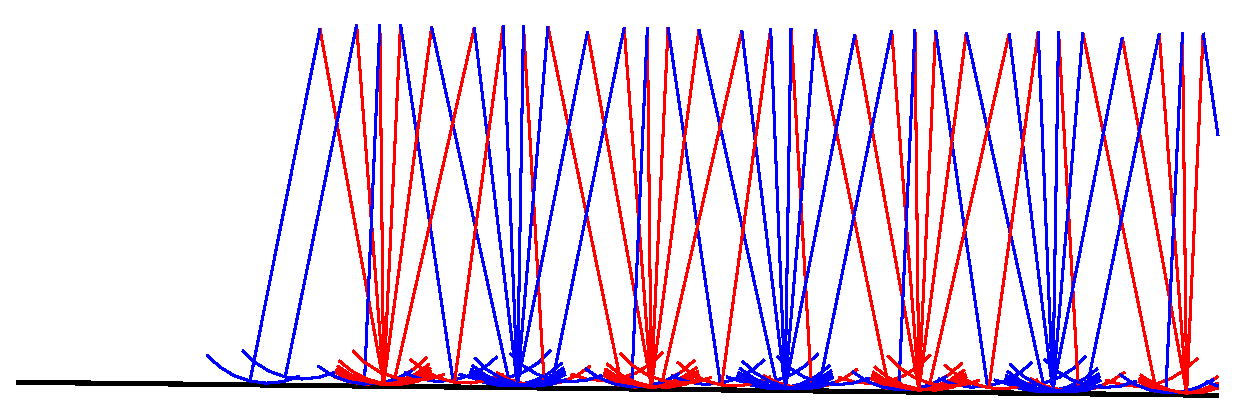
\includegraphics[width=3in]{\figurepath/passive_walking.eps}
\caption{Stable passive walking gait}
\label{fig:passive_walk}
\end{figure}
Figure \ref{fig:passive_walk} shows the gait of the passive walker. 
After coupling the neural oscillator, the basic pattern is not changed  as shown in \figurename ~\ref{fig:stable_active_walk}.

\begin{figure}[H]
\centering
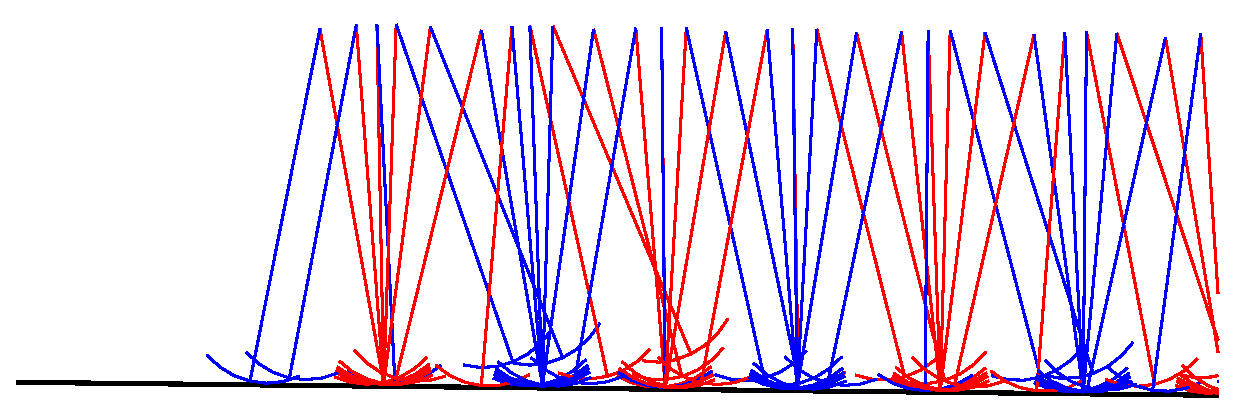
\includegraphics[width=3in]{\figurepath/actuated_walk_downslop.eps}
\caption{Walk down the same slop when actuated}
\label{fig:stable_active_walk}
\end{figure}

\textbf{Walking On Plain}
However the stability is fragile.  
The passive walker can't walk on plane. 
The step size will decrease after each step, and finally it will stop or fall over as illustrated in \figurename ~\ref{fig:pass_waling_on_plane}.
\begin{figure}[!h]
\centering
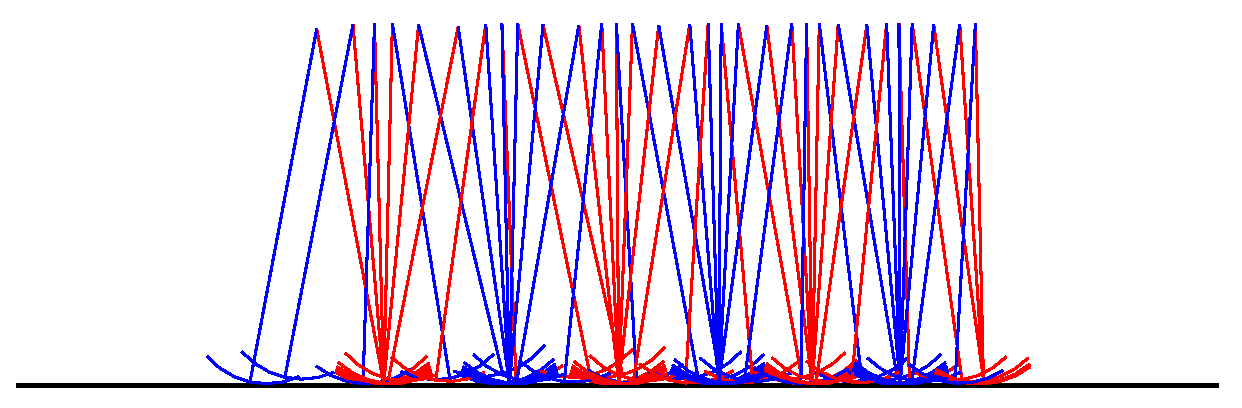
\includegraphics[width=3in]{\figurepath/passive_walk_on_plane.eps}
\caption{Passive walking gait can't be maintained on plane}
\label{fig:pass_waling_on_plane}
\end{figure}

After coupled with the neural oscillator, this walking machine can walk on plane, and exhibits gait similar to the passive dynamic walker. 
\figurename ~\ref{fig:walk_plane} shows the gait. 
From the state plot \figurename ~\ref{fig:walk_plane_state}, and phase plot \figurename ~\ref{fig:walk_plane_phase}, we can see that the gait converged to a stable limit circle.


\begin{figure}[!h]
\centering
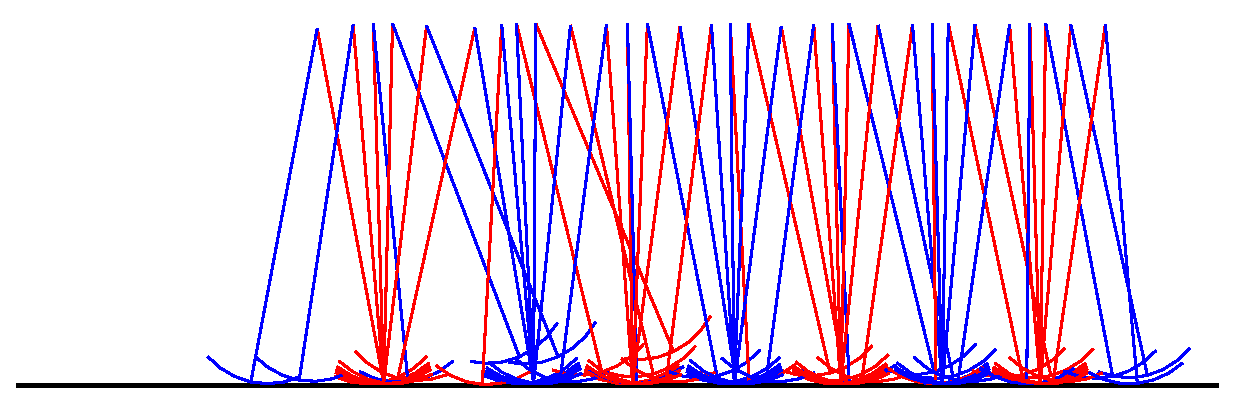
\includegraphics[width=3in]{\figurepath/walker_on_plane.eps}
\caption{Walking on plane under neural control}
\label{fig:walk_plane}
\end{figure}


\begin{figure}[!h]
\centerline{
\subfigure[State Plot]{
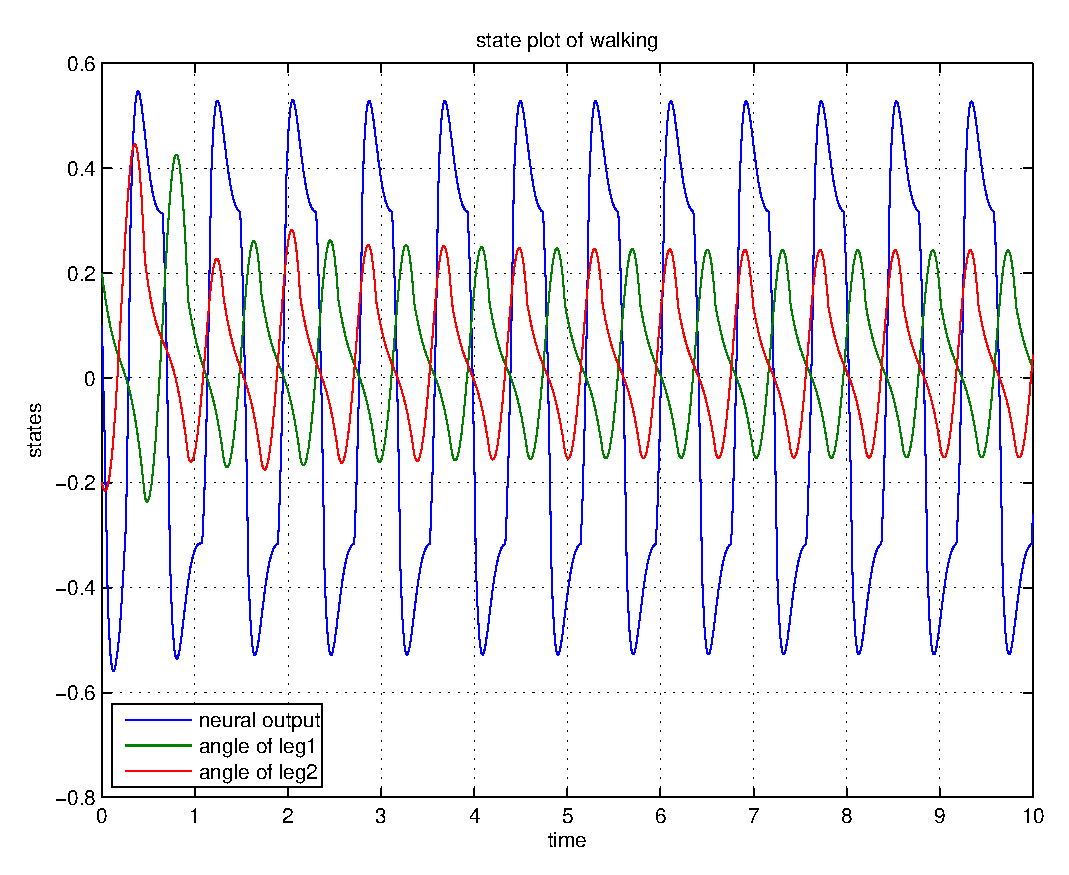
\includegraphics[width=1.5in]{\figurepath/walking_on_plane_time_state}
\label{fig:walk_plane_state}
}
\hfill
\subfigure[Phase Plot]{
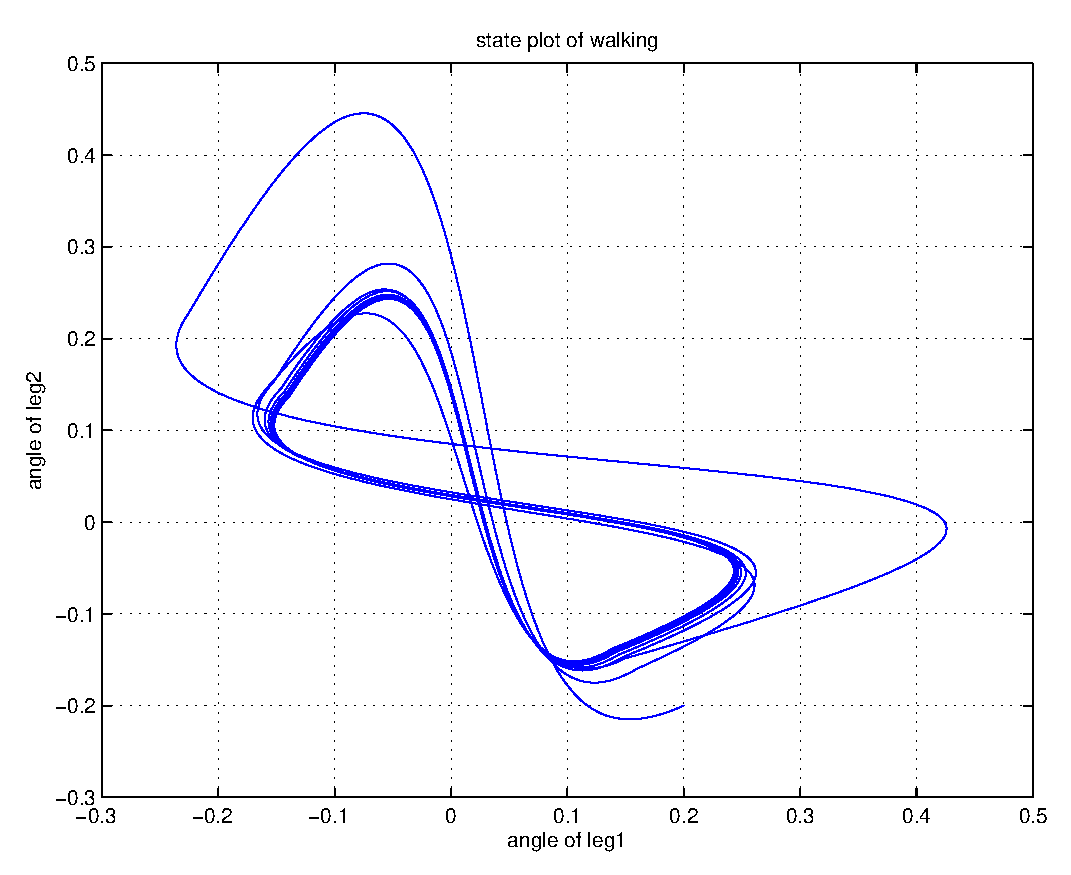
\includegraphics[width=1.5in]{\figurepath/walking_on_plane_phase.eps}
\label{fig:walk_plane_phase}
}
}
\caption{
Walking on a plane converges to a stable limited circle
}
\label{fig:walk_on_plane}
\end{figure}

To verify the structural stability, we introduce a variety of perturbations to the passive walker. 
These perturbations include different initial condition, different slopes, different leg mass and different leg length.

\textbf{Different Initial Condition}
The original passive walker is not very stable. 
A slight change in initial condition will result in walking failure. 
While after coupled with neural oscillator, the basin of attraction has been enlarged. 
A different initial condition can still lead to a stable gait, as show in Figure \ref{fig:diff_init}. 
Natural looking gait is maintained.
\begin{figure}[h]
\centering
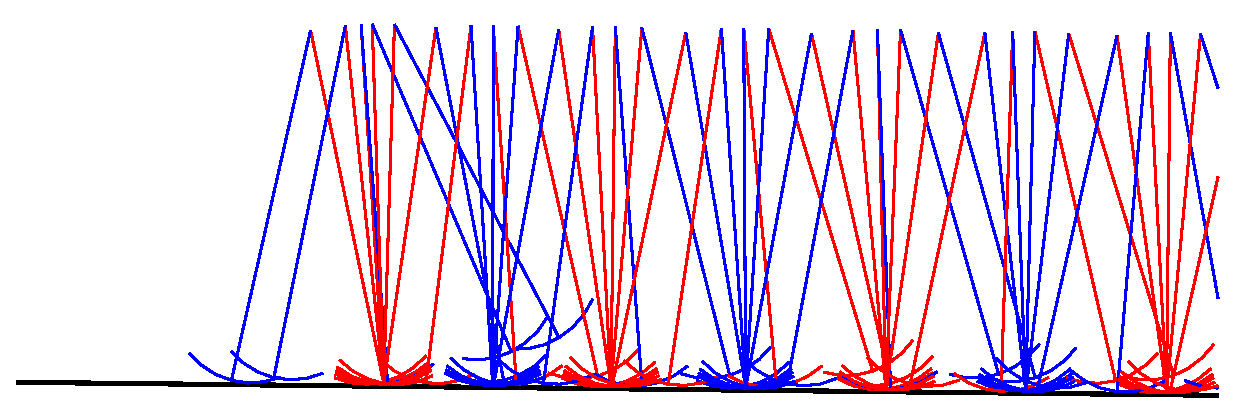
\includegraphics[width=3in]{\figurepath/walk_down_with_differnt_init_cond_suceed.eps}
\caption
{
Walking with different Initial condition
}
\label{fig:diff_init}
\end{figure}
 

\textbf{Walking On Different Slopes}
Another parameter we change is angle of the walking slope. 
When we increase the down slope, stable walking motion can still be maintained, as shown in figure \ref{fig:diff_slop}.
An important discovery is that although the walkers can walk on various down slopes, it can not walk up slope,no matter how control parameters are changed.
It can’t walk up slope and will fall backward after several steps. 
We suggest that this is because the proper limit circle does not exist in the dynamic system when walking up slope.
This finding may help us to understand the upper body effect in walking.

\begin{figure}[h]
\centering
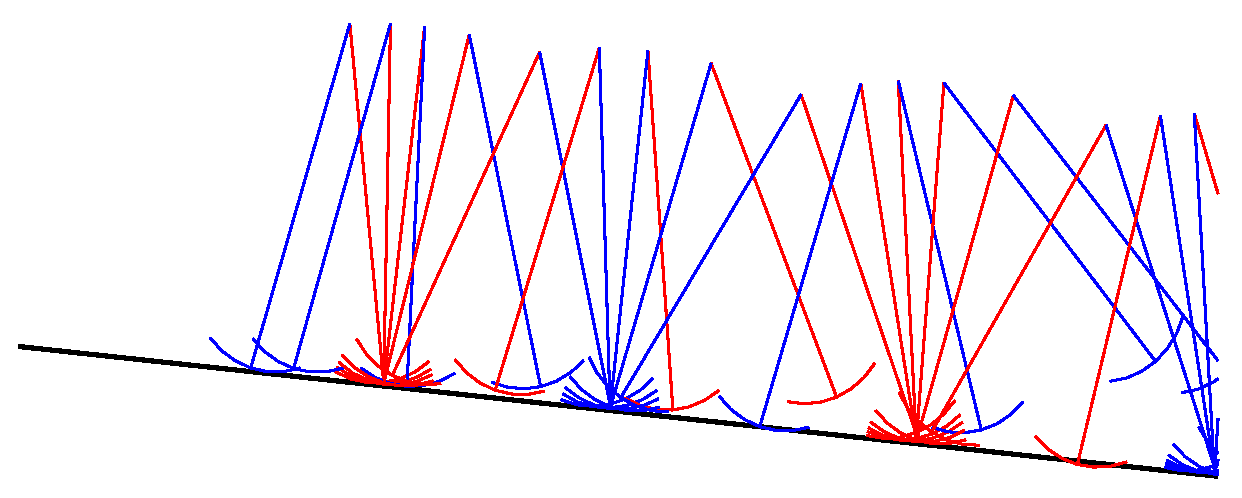
\includegraphics[width=3in]{\figurepath/big_slop_actuated_suceed.eps}
\caption
{
Walking with different slope angle
}
\label{fig:diff_slop}
\end{figure}

\textbf{Leg Mass Variation}
We add mass on one leg to 50\% and find the stability of the gait is still maintained. 
The step length and swing period of the two legs are different, this gait is similar to that with a crippled leg, see figure\ref{fig:leg mass}.

\begin{figure}[H]
\centering
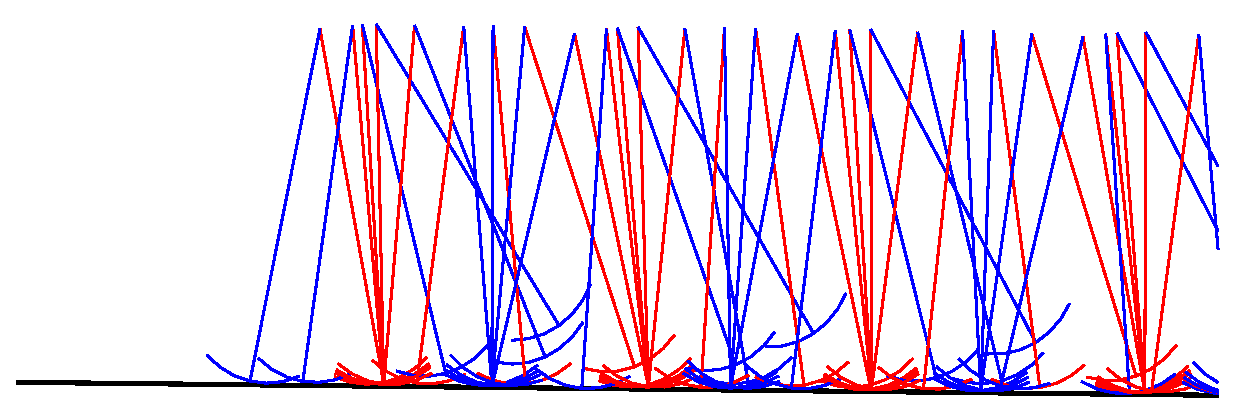
\includegraphics[width=3in]{\figurepath/walk_mass_changed.eps}
\label{fig:walk_mass_changed}
\caption
{
Walking with legs of different mass
}
\label{fig:leg mass}
\end{figure}

\textbf{Leg Length Variation}
The last parameter we change is the leg length. 
We change the leg length to 1/8 shorter. 
And we find the stability of the gait is maintained, see \figurename ~\ref{fig:walk_leg_changed}

\begin{figure}[H]
\centering
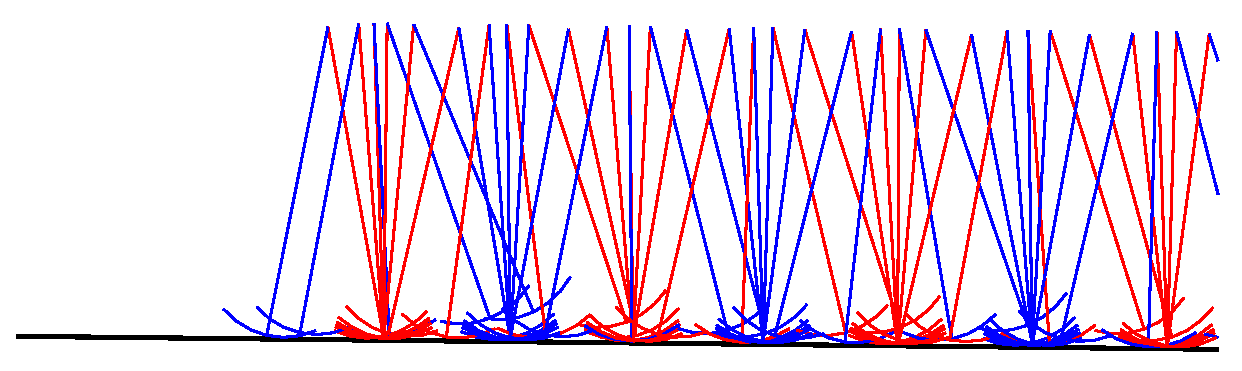
\includegraphics[width=3in]{\figurepath/walk_leg_changed_success.eps}
\caption
{
Walking with shorter Legs
}
\label{fig:walk_leg_changed}
\end{figure}






\section{Discussion and Future Work}
Qualitative Control Theory can synthesize motion with adaptive behaviour while keeping the qualitative properties of motion.
It provides a new method to synthesize adaptive motion efficiently. Since very little computation involved in each controller, compared with traditional optimiaztion based method, this method can generate motions in realtime. And most importantly, our method is parallel in nature. Each CPG only control on single degree of freedom. For complicate characters, many different CPGs can be simulated in parallel without referencing each other. Since many physical simulation modules have been implemented efficiently using GPU, in future, most of the computational burden of our method can be shifted to GPU. This will make our algorithm generating agile motions even with very complicated environment and involving whole body structures. 


However since we bring in a new theory into the motion synthesis area, many works need to be done in the future. For example, our current model only involves the lower body structure, upper body and more joints will be considered in our future design. To proof the adaptivness, we will need experiment on more complicate terrian instead of just upslope and downslope.

More Central Pattern Generators are needed for different kinds of motions. And how to turn the CPG parameters for the animator purpose are still open.
These topics will be covered in the future research.







\bibliographystyle{plainnat}
\bibliography{rommePaper}




\end{document}


